\chapter{Preliminaries}
\label{cha:Preliminaries and Definitions}

This chapter present notations and definitions that will be used throughout the thesis.

\section{Definitions}
Informally an entity is \emph{negligible} if it is too small to matter \cite{commitment}.

\begin{mydef}[Negligible]
$\epsilon(k)$ is negligible in $k$ for any positive polynomial $p$ where $\epsilon(k)\leq\frac{1}{p(k)}$ for all large enough k. 
% that is k and what is epsilon?
\end{mydef}

A distinguisher $D$ plays a game where two probabilistic algorithms $U$ and $V$ run on the same input $x$. $D$ gets $x$ and now has to guess if the output $y$ is generated from $U$ or $V$ on input $x$. The output  distributions of $U$ and $V$ on input $x$, this will be refereed to as $U_x$ and $V_x$.

\begin{mydef}[Statistical Distance]
Given two probability distributions, $P$ and $Q$, the statistical distance between them is defined as $SD(P,Q)=\frac{1}{2}\sum_{y}|P(y)-Q(y)|$, where $P(y)$ is the probability $P$ assigns to $y$.
\end{mydef}
17


\begin{mydef}[Statistical indistinguishable]
Given two probabilistic algorithms $U$ and $V$ they are statistical indistinguishable if $SD(U_x, V_x)$ is negligible in the length of the string $x$. We write this $U \textasciitilde^s V$.
\end{mydef}

\section{Notation}
% MPC notation and vague definition of secure = privacy + correctness.
% From MPC BOOK
The parties or players that participate in the execution of the protocol are called $P_1, P_2,...,P_n$. Each player $P_i$ holds a secret input $x_i$ and the agreed function takes $n$ inputs. The goal is to compute $y=f(x_1, x_2,...,x_n)$ while making sure that the \emph{correctness} of the protocol is satisfied, meaning that the correct value of $y$ is computed. Furthermore, it is required that there is \emph{privacy}, meaning that $y$ is the only new information released. Computing $f$ such that privacy and correctness are satisfied is refereed to as computing $f$ \emph{securely}. 
When you want to look at the security of a protocol you do it with regards to some adversary attacking. Loosely speaking we define a protocol execution in an \emph{ideal world}, where the protocol is executed in an ideal and secure way. The protocol execution in the ideal world is then compared to a protocol execution in the \emph{real world}. Then for all adversaries there exists a simulator, so that the adversary in the real game and the simulator in the ideal game achieve the same effect. Any attack that is done in the ideal world can also be done in the real world, but in the ideal world we have something ideal and secure and thus the affect of any attack in the ideal world is acceptable. Hence we are happy if any attack achieve the same affect in the real world. 
It is now clear what we must look at the capabilities of the adversary attacking the protocol.

\section{Adversaries} 
% file:///C:/Users/koller-desktop/Downloads/Multiparty_Computation_an_Introduction.pdf

In MPC protocols multiple players can be corrupted. $C$ is the set of corrupted players and $t$ the maximum number of parties that is allowed to be corrupt whilst security can still be guaranteed. Think of an adversary as a malicious entity which can corrupt a subset of players and which aim to prevent the users of the protocol to achieve their goal. All the corrupted parties could cooperate or be controlled by one entity and therefore a single adversary is modelled to control all corrupted parties\cite{mpc-book}.

\begin{mydef}[Passive adversary]
A passive adversary obtains the complete information obtained by the corrupted players but the players still follow the protocol as specified. It will use the information to try to learn more than it should.
\end{mydef}

\begin{mydef}[Active adversary]
An active adversary take full control of the corrupted players and does not need to follow the protocol as specified.
\end{mydef}

An adversary can also vary how he corrupts the players. Both passive and active adversaries can be static or adaptive.

\begin{mydef}[Static adversary]
For a static adversary the set of corrupted players are set before the protocol starts and will remain the same throughout the execution of the protocol.
\end{mydef}

\begin{mydef}[Adaptive adversary]
An adaptive adversary can at any time during the protocol choose to corrupt new players.
\end{mydef}

\section{Communication} 
We will also model what the adversary is allowed to do communication-wise.

\begin{mydef}[Synchronous model]
In the synchronous model there is clocks that are synchronized such that when a message is sent it will arrive before some time bound. We assume that there is pairwise secure channels, such that the adversary cannot interfere with the network traffic.
\end{mydef}

\iffalse % TODO mayne introduce simulation
\section{The Simulation Paradigm}
The UC Model 
The idea that the protocol can be efficiently simulated without interacting with any parties. We therefore introduce a simulator $S$ and give it the power to do the protocol steps in any order it wants.
\fi

\section{Privacy and Robustness} 
We also define what the players are \emph{allowed} to do and see, as well as what they \emph{actually} can do and see during an execution of a protocol\cite{mpc-book}.

\begin{mydef}[Leaked Values]
The leaked values $\{view_j\}_{P_j \in C}$ are exactly the information leaked to the corrupted parties during an execution of the protocol.
\end{mydef}

\begin{mydef}[Allowed Values]
The allowed values $\{x_j,y_j\}_{P_j \in C}$ are the corrupted players own input and output that they will learn during the execution of the protocol.
\end{mydef}

%Privacy
Intuitively, a protocol is private if the leaked values contain no more information than the allowed values. In cryptography you often rely on hard problems were no polynomial time algorithm is known to solve the problem. Therefore it makes sense to say that a protocol is private if the leaked values can be computed efficiently from the allowed values. The program that efficiently computes the leaked values from the allowed values is called a simulator $S$. Since parties in MPC protocols can make random choices it is defined that:

\begin{mydef}[Privacy]\label{def:privacy}
A protocol is private if there exists an efficient simulator $S$ such that the simulated values $S(\{view_j\}_{P_j \in C})$ and the leaked values $\{view_j\}_{P_j \in C}$ have the same distribution.
\end{mydef}

%Robustness
We define robustness of a protocol to model the influence an active adversary has on the output of a protocol.
The influence an attacker has on the protocol execution, we call the \emph{actual influence} and the influence we allow we call the \emph{allowed influence}. We reuse the approach from privacy as define robustness as such:

\begin{mydef}[Robustness]
A protocol is robust if there exists an efficient simulator $S$ such that for every adversary attacking the protocol, $S$ can efficiently compute an allowed influence with the same effect.
\end{mydef}

%Combine
We require one single simulator that simultaneously can demonstrate both privacy and robustness.

\section{The UC Model} 
The Universally Composable (UC) Model describes security for a cryptographic protocol $\pi$. In this model a protocol can be proven secure regardless of the context. We will model protocols through interactive systems and interactive agents\cite{mpc-book}.

\begin{mydef}[Interactive agent (IA)]
An interactive agents is a computational device that receives and sends messages on named ports and that holds an internal state.
\end{mydef}

\noindent A set of interactive agents can become an \emph{interactive system} (IS) by connecting the in-port and out-ports with the same name as seen in \ref{fig:IA_IS}

\begin{figure}[H]
    \centering
    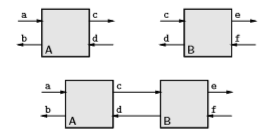
\includegraphics{images/Interactive_systems.PNG}
    \caption{
    An interactive agent $A$ with $In(A)={a,d}$ and $Out(A)={b,c}$. \\
    An interactive agent $B$ with $In(B)={c,f}$ and $Out(B) = {d,e}$. \\
    And the interactive system $IS=A \diamond B$ with $Out(IS)={a,f}$ and $In(IS)={b,e}$. %MPC BOOK
    }
    \label{fig:IA_IS}
\end{figure}

\begin{mydef}[Behavioral Equivalence]
Two interactive systems having different internal structure are behavioral equivalent if they are indistinguishable for and outside observer, meaning that they give the same outputs on the same open out-ports whenever they get the same input on the same open in-ports. 
\end{mydef}

\subsubsection{Ideal Functionality}
Imagine an ideal world with an ideal protocol. This ideal protocol is a specification of what we could like the real protocol to do. In the ideal world we model the protocol as an interactive agent and call this an \emph{ideal functionality} $F$. In the real world the model the protocol $\pi$ as an interactive system and then the goal is to proof that $\pi$ is at least as secure as $F$, by showing that they are \emph{behavioral equivalent}.

% How does F work for secure function evaluation
For secure function evaluation $F$ informally will work as such: All the players will give their input to $F$ that will always calculate the correct result according to its specification, without leaking any information other than the outputs it is supposed to send to the players. $F$ has an input and output port for every player. Further more it has two special ports called the leakage port and influence port that is used for communication with the adversary. When a protocol is executed the in-ports and out-ports are used, but if a player $P_i$ is corrupted then $F$ stops using the $i$'th in/out-ports and use instead the leakage and influence port, where adversary then will communicate on behalf of $P_i$.

\subsubsection{The environment}
$\pi$ and $F$ should be equivalent no matter the context. The protocol could fx. be used as a subroutine in a bigger system, that is  part of an environment. The environment can be modelled as an interactive system that choose inputs of the players and use the protocol and receive the result from the protocol. We denote the environment as $Z$. The environment get two play with with either $pi$ or $F$ and the it should not be able get guess which one in is, except with negligible probability close to ½.

\section{Secret Sharing}
Secret sharing is a method for distributing a secret to multiple parties who each get a share of the secret that reveals nothing about the secret. The secret can be reconstructed when a sufficient number of shares are combined together.

\subsubsection{Lagrange Interpolation}
Given a set $C$ of size $m$ consisting of $t+1$ or more points that are evaluations of some polynomial $f$ of degree $t$, then we can compute any point on the polynomial as such:

\begin{align*}
    f(x) = \sum_{i \in C} f(i) \delta_i(x) 
\end{align*}

\noindent where $\delta_i$ is
\begin{align*}
    \delta_i(x)=(\prod_{j \in C, j \neq i} \frac{x-j}{i-j})
\end{align*}

Note that one can construct a recombination vector $\boldsymbol{r_j}=(r_1^j,...,r_m^j)=(\delta_1(j),...,\delta_m(j))$ that can be used to compute the value $f(j)$. This recombination vector works for all polynomials of degree lower than $m-1$.

\subsection{Shamir's Secret Sharing Scheme}
This scheme is based on polynomials over a finite field $\mathbb{F}$. To share a secret $s \in \mathbb{F}$ a dealer has to choose a random polynomial $f_s$ over $\mathbb{F}$ of degree at most $t$ where $f_s(0)=s$. Then $n$ shares are generated by evaluating $f_s$ on the points $f_s(1),...,f_s(n)$. The $n$ shares can then be privately distributed to the $n$ parties. This works because any set of $t$ or fewer shares contain no information on $s$, but if you have $t+1$ or more shares the polynomial can be reconstructed by using Lagrange Interpolation. This means that if $t$ or less corrupt parties goes together and pool their information they can gain no extra information about the secret $s$. 

A secret sharing can be defined as a vector:

\begin{align*}
    [s;f_s]_t = (f_s(1), f_s(2), ..., f_s(n))
\end{align*}

Note that this notation states that $deg(f_s) \leq t$, $f_s(0)=s$ and it describes the shares $(f_s(1), f_s(2), ..., f_s(n))$. The notation will vary between $[s;f_s]_t=[s;f_s]=[s]$. 
% TODO maybe just stick to [s;f_s]_t

We can do arithmetic operations on the shared secrets by using entry wise addition, scalar multiplication and Schür product on the shares as such:

\begin{align*}
    [a;f]_t + [b;g]_t &= (f(1) + g(1), ... , f(n) + g(n)  &=& [a+b; f+g]_t\\
    \alpha [a;f]_t &= (\alpha(1), \alpha f(2), ... , \alpha f(n) &=& [\alpha a; \alpha f]_t\\
    [a;f]_t * [b;g]_t &= (f(1) * g(1), ... , f(n) * g(n) &=& [ab;fg]_{2t}
\end{align*}

\section{Algebra}
In the MPC protocols explored in this thesis computations are done in a field $\mathbb{F}$, because they use Shamir's Secret Sharing. This means that the input from the player must be elements in the field and the result will also be an element in the field. Hence, we need to understand how to do arithmetic in a field. To understand this we need understanding of algebraic structures such as groups, rings and fields\cite{algebra}.

\subsection{Groups}
A pair $(G, \circ)$ consisting of a set G and a composition $\circ$ is called a group if it satisfies the following properties:

\begin{enumerate}[(i)]
    \item The composition is associative: $a \circ (b \circ c) = (a \circ b) \circ c$ \\
    for every $a, c, b \in G$. 
     \item There is a neural element $e \in G$ such that: $e \circ a = a$ and $a \circ e = a$ \\
    for every $a \in G$. 
     \item For every $a \in G$ there is an inverse element $t \in G$ such that $t \circ a = e$ and $a \circ t = e$.
\end{enumerate} 
\noindent A group $G$ is called abelian if $a \circ b = b \circ a$ for every $a, b \in G$. For any natural number $n$, $(Z_n, +)$ is a group where $+$ means addition modulo $n$. For multiplication the neutral element is $1$ and thereby $(Z_n, \cdot)$ is not a group because $0$ does not have an inverse. $(Z_n\backslash \{0\}, \cdot)$ is also not a group. If you look at the element $2 \in Z_6$ and multiply it with any number in $Z_6$ you would get an even number, and thereby not the neutral element $1$ and thereby we see that there is no inverse of $2 \mod 6$. The solution to making multiplication modulo $n$ be a group operation is to get rid of all the the numbers where $gcd(a,n) \neq 1$.

\begin{align*}
     Z^*_n=\{a \in Z_n\ |\ gcd(a,n)=1\}
\end{align*} 

\subsection{Rings}
A ring is an abelilian group $(R, +)$ with an additional composition called multiplication. Multiplication satisfies the following for every $a,b,c \in R$: 

\begin{enumerate}[(i)]
    \item $a \cdot (b \cdot c) = (a \cdot b) \cdot c$
    \item There is a neural element $1 \in R$ such that: $1 \cdot a = a$ and $a \cdot 1 = a$ 
    \item $a \cdot (b + c) = a \cdot b + a \cdot c$ and $(b + c) \cdot a = b \cdot a + c \cdot a$ 
\end{enumerate}

\subsection{Fields}

A field is a ring $R$ such that the second operation also satisfies all group properties. i.e $R^* = R \setminus \{0\}$ is called a field. A finite field also called a Galois field only exists if $|\mathbb{F}| = p^n$. where p is a prime and $n \geq 1$. When we write $GF(q)$ we mean a finite field of size q. For example $GF(11)$, here $p=11$ and $n=1$ so this is fine. Another example is the binary field $GF(256)$=$GF(2^8)$. If $n=1$ then we have a prime field $GF(p)$ and if $n > 1$ then we have an extension field. 

\subsubsection{Prime Field Arithmetic}  
 Elements of a prime field $GF(p)$ are the integers $\{0,1,...,p-1\}$. For $a,b \in GF(p)$. For $a,b \in GF(p)$ arithmetic's are done in the following way:

\begin{enumerate}[(i)]
    \item Addition: $a+b\ \equiv c \mod p$
    \item Subtraction: $a-b \equiv d \mod p$
    \item Multiplication: $a \cdot b \equiv e \mod p$
    \item Inversion: The Inverse $a^{-1}$ must satisfy $a \cdot a^{-1} \equiv 1 \mod p$. So how do we compute $a^{-1}$? It can be computed with the extended Euclidean Algorithm.
\end{enumerate}

\subsubsection{Extended Field Arithmetic}
In cryptography we are interested in fields where $GF(2^n)$. The elements of $GF(2^n)$ are  polynomials $a_{n-1} \cdot x^{n-1} +...+a_1 \cdot x + a_0 = A(x) \in GF(2^n)$, where the coefficients $a_i \in GF(2)=\{0,1\}$. An example is $GF(2^3)$, were we know that any element must have the form $A(x)=a_2 x^2 + a_1 + a_0$. We can view that as a 3 bit vector and we can express 8 different numbers with with 3 bits which makes sense since we are working with $GF(2^3)=GF(8)$. The elements in the group is $GF(8)=\{0,1, x, x+1, x^2, x^2+1, x^2+x, x^2+x+1$\}.
In an extension field $A(x),B(x) \in GF(2^m)$ with the coefficients $a_i$ and $b_i$ addition is by regular polynomial addition:

\begin{align*}
      &C(x) = \sum_{i=0}^{n-1} c_i \cdot x_i \text{, where } c_i \equiv a_i+b_i \mod 2
\end{align*}

\noindent So just add or subtract the coefficients of the polynomials in $GF(2)=\{0,1\}$. Addition in $GF(2^3)$ with the elements $A(x)=x^2+x+1$ and $B(x)=x^2+1$ would be:

\begin{align*}
    A(x) + B(x) &= ((1+1) \mod 2) x^2 + x + ((1+1) \mod 2) \\
    &= 0 x^2 + x + 0 \\
    &= x
\end{align*}

\noindent For multiplication in $GF(2^m)$ one might think that you can do regular polynomial multiplication as such:

\begin{align*}
    A(x) \cdot B(x) &= (x^2 + x + 1) \cdot  (x^2 + 1) \\
    &= x^4 + x^3 + x^2 + x^2 + x + 1 \\
    &= x^4 + x^3 + ((1+1) \mod 2) x^2 + x + 1 \\
    &= x^4 + x^3 + x + 1 = C'(x)\\
\end{align*}

\noindent Here we have a problem since $C'(x) \not\in GF(2^3)$. The solution is to reduce $C'(x)$ modulo a polynomial that "behaves like a prime" in the sense that the polynomial can not be factorized. These are called irreducible polynomials. An irreducible polynomial for $GF(2^3)$ is $P(x)=x^3+x+1$. Let $A(x)$,\ $B(x) \in GF(2^m)$ and let $P(x) \equiv \sum_{i=0}^m p_i x^j$, where $p_i \in GF(2)$ be an irreducible polynomial, then multiplication is performed as $C(x) \equiv A(x) \cdot B(x) \mod  P(x)$. If we for example look at the earlier example we get: $\dfrac{x^4 + x^3 + x + 1}{x^3+x+1}$. First we want to get rid of $x^4$, so we multiply $P(x)$ by $x$ and we get $x^4+x2+x$ and then we add it to $A(x) \cdot B(x) = C'(x)$:

\begin{align*}
    C'(x) + (P(x)*x) = (x^4 + x^3 + x + 1) + (x^4+x2+x) = x^3+x^2+1 
\end{align*}

 \noindent but this is still not in our field so we reduce again, but only with p(x) this time because we already got rid of $x^4$.
 
 \begin{align*}
    (x^3+x^2+1) + (x^3+x+1) &= x^2 + x \in GF(2^3)
\end{align*}

\noindent Now we have an element in our field and we have done. \\ 
For every field $GF(2^m)$ there are several irreducible polynomials and the result of the arithmetic in the fields depends on that irreducible polynomial is being used. In AES the irreducible polynomial used is $P(x)=x^8+x^4+x^3+x+1$.

In $GF(2^m)$ again the inverse $A^{-1}(x)$ of an element $A(x) \in GF(2^m)$ must satisfy that $A(x) \cdot A(x)^{-1} \equiv 1$ and what we again use to find it is the extended Euclidean Algorithm.

\section{Van der Monde Matrices}

\begin{mydef}[Invertible matrice]
An $n \times n$ square matrix $A$ is \emph{invertible} if there exist another $n \times n$ matrix $B$ such that: $AB=BA=I$, where $I$ is the identity matrix. If the determinant of a square matrix is $0$ then it has no inverse.
\end{mydef}

A Van der Monde matrix with $r$ rows and $c$ columns is a matrix is on the form:

\begin{align*}
\begin{bmatrix}
    1       & x_1^1     & x_1^2     & \dots     & x_1^{c-1} \\
    1       & x_2^1     & x_2^2     & \dots     & x_2^{c-1} \\
    \vdots  & \vdots    & \vdots    & \ddots    & \vdots    \\
    1       & x_r^1     & x_r^2     & \dots     & x_m^{c-1} \\
\end{bmatrix}   
\end{align*}

We use the notation $Van^{(r,c)}$ for a Van der Monde matrix with $r$ rows and $c$ columns, where all the elements $x_1, ... ,x_n$ are distinct. If all numbers in a sqaure Van der Monde matrix are distinct then the determinant is non-zero and thereby it has an inverse. 
For a matrix $M=Van^{(r,v)}$ with $r>c$ we can create a new matrix $M_r$ from the subset of the rows $R\subseteq\{1,...,r\}$ where $|R|=c$. This matrix will also be invertible as it is a square Van der Monde matrix. This means that we can choose any $c$ rows from $M$ and get an invertible matrix. We say that the matrix is \emph{super-invertible}.

\subsection{Secret Sharing}
A secret sharing $[s;f_s]_t$ can be done with Van der Monde matrices by constructing a Van der Monde matrix that can evaluate polynomials when multiplied with a vector of points. In the vector we set $x_0=s$ and $(x_1\dots x_t) \in_R \mathbb{F}$.

\begin{align*}
    &M^{(t)} &= Van^{(n,t+1)}(1,\dots,n) \\
    &M^{(t)} \cdot (x_0,\dots,x_t) &= (f_s(1), f_s(2), ..., f_s(n))
\end{align*}

\noindent Normally when we do Shamir's secret sharing with with $[s;f_s]_t$ we evaluate a polynomial on a point for each player and disribute $f_s(x_i)$ to player $P_i$. For example:
\begin{align*}
    &f(x) = 5x^2+4x+3, \quad f(1)=12, f(2)=31, f(3)=60 \\
\end{align*}

\noindent It is easy to see that we can acheive the same with a Van Der Monde matrix:

\begin{align*}
    &M^{(2)} \cdot (x_0, x_1,x_2) =
    \begin{bmatrix}
    1       & 1     & 1^2  \\
    1       & 2     & 2^2 \\
    1       & 3     & 3^2 
    \end{bmatrix}  
    \begin{bmatrix}
    3        \\
    4        \\
    5        
    \end{bmatrix} =
    \begin{bmatrix}
    12        \\
    31        \\
    60        
    \end{bmatrix} 
\end{align*}



\subsection{Randomness Extraction}
Van der Monde Matrices can be used for randomness extraction. For $M=Van^{(r,c)^\intercal}$ with $r>c$. We can compute $M\cdot(x_1,\dots,x_r)=(y_1,\dots,y_c)$ and extract randomness from the vector $X=(x_1,\dots,x_r)$, even when only $c$ of the $x$ values are chosen uniformly random. 

\begin{align*}
    \underset{(c \times r)}{M} \cdot \underset{(r \times 1)}{X} =
    \underset{(c \times 1)}{Y}
\end{align*}

\noindent To see this we denote $M^R$ to a square matrix for some subset of $c$ rows, that we multiply with a vector $X^R$ with $c$ uniformly random chosen values of $x_i$'s. 

\begin{align*}
    \underset{(c \times c)}{M^R} \cdot \underset{(c \times 1)}{X^R} =
    \underset{(c \times 1)}{Y^R}
\end{align*}

\noindent Since $M^R$ is inevitable and the vector $X^R$ by definition is uniformly random we get that theot vector $Y^R$ is uniformly random.
We denote $M^T$ to be matrix with the $t$ rest of the rows in $M$ that is not in $M^R$ and multiply it with a vector $X^T$ with $t$ values $x_j$ that is not uniformly random, but still chosen independently from the $x_i$'s.
    
\begin{align*}
    \underset{(c \times t)}{M^T} \cdot \underset{(t \times 1)}{X^T} =
    \underset{(c \times 1)}{Y^T}
\end{align*}

Now we have that $M \cdot R=Y^R+Y^T=Y$, where $Y^R$ is uniformly random and $Y^T$ is chosen independently from $Y^R$ and thus $Y$ is uniformly random.

\section{Circuits}
Secure Function Evaluation protocols can evaluate any function $f$ with $i$ inputs and $j$ outputs, where $i$ and $j$ are positive integers. We look at protocols where the mapping $f(x_1,x_2,...,x_i)=y_1,y_2,...,y_j$ is be described using a arithmetic circuit.

An arithmetic circuit is an acyclic direct graph where each node is a gate and each gate has input wires and output wires. There is $i$ input gates with no incoming wires and any number of outgoing wires. The players knows on forehand which gate they have to supply their secret input. There is $j$ number of output wires with with one input wire and one output wire. Internally there can be addition and multiplication gates which both has two input wires and one output wire. There is also multiply-by-constant gates what was one input wire and one output wire. Evaluating a circuit can be done first evaluating all circuit in the first layer of the circuit and then the next layer and then repeat until all layers has been evaluated. 
Boolean circuits are like arithmetic circuits, except the internal gates can be an and-gate, or-gate, xor-gate or a not-gate. Furthermore the inputs and outputs are bits. If you want to evaluate a boolean circuit with an SFE protocol for arithmetic circuits it can be done by emulatation. This means using the analytical representations of boolean gates. 
$f(a) = 1-a$ is the analytical representation of a NOT gate:
     \begin{itemize}
        \item f(0) = 1-0 = 1
        \item f(1) = 1-1 = 0
    \end{itemize}
$f(a,b) = a*b$ is the analytical representation of an AND gate:
    \begin{itemize}
        \item f(0,0) = 0*0 = 0
        \item f(0,1) = 0*1 = 0
        \item f(1,0) = 1*0 = 0
        \item f(1,1) = 1*1 = 1
    \end{itemize}
$f(a,b) = (1-(1-a)(1-b)) = a + b - a*b$ is the analytical representation of an OR gate:                   \begin{itemize}
        \item f(0,0) = 0+0 - 0*0 = 0
        \item f(0,1) = 0+1 - 0*1 = 1
        \item f(1,0) = 1+0 - 1*0 = 1
        \item f(1,1) = 1+1 - 1*1 = 1
    \end{itemize}
$f(a,b) = a + b - 2*a*b$ is the analytical representation of an XOR gate, since the XOR it addition without a carry $a+b$ is the addition in first position and $-2ab$ removes the carry in second position.
    \begin{itemize}
        \item f(0,0) = 0+0 - 2*0*0 = 0
        \item f(0,1) = 0+1 - 2*0*1 = 1
        \item f(1,0) = 1+0 - 2*1*0 = 1
        \item f(1,1) = 1+1 - 2*1+1 = 0
    \end{itemize}


